\section{Method}

\begin{figure*}[th]
    \centering
    \scalebox{1}{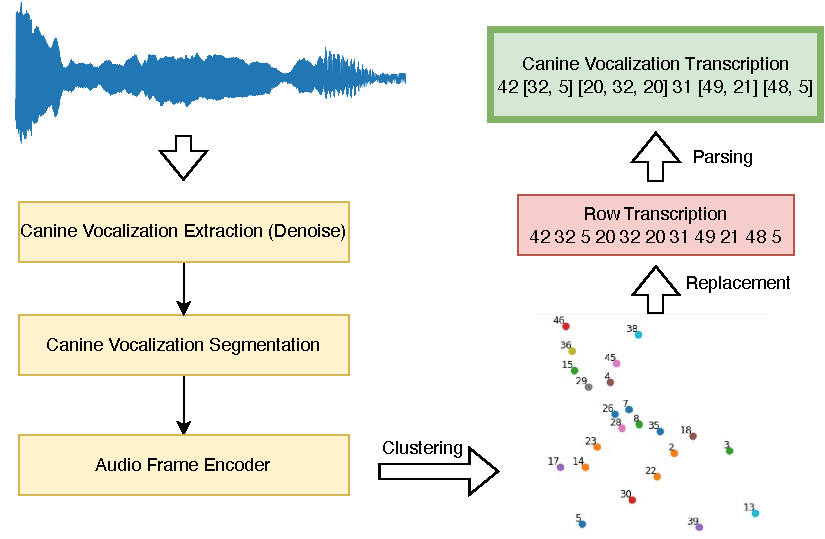
\includegraphics{sys_1.pdf}}
    \caption{Transcription Example}
    \label{fig:sys1}
\end{figure*}

We present some technical details under the hood of this interactive canine lexical analysis system system. The method presented here are only preliminary, ``various components'' of this pipeline can be replaced and updated. To mitigate issues related to poor audio quality and severe noise contamination resulting from large datasets, we utilized deep learning-based audio denoising and audio event detection techniques to obtain the final canine sound sentences. Clustering was employed to label each audio frame, resulting in the identification of 36 canine sound phonemes and 14 noise phonemes, after manual filtering due to noise presence among the 50 phonemes. We designed and calculated the plausible score for each N-gram using NLP algorithms, obtaining the canine sound vocabulary, and subsequently utilized parsing algorithms to generate the final transcription of canine language. The whole pipeline is shown as \figref{fig:sys1}.

\subsection{Phoneme Clustering}

To obtain the phonemes in a sentence in the dog language, we use methods including audio clean-up by AudioSep, sentence extracting and phoneme recognition.

\paragraph{Audio Clean-up by AudioSep.} To separate dog sounds from audios that contain both dog sounds and noises, we apply AudioSep~\citep{liu2023separate}, a audio source separation model that has been pre-trained on large-scale multimodal datasets, including AudioSet~\citep{gemmeke2017audio} dataset, VGGSound~\citep{chen2020vggsound} dataset, AudioCaps~\citep{kim2019audiocaps} dataset, etc. We apply PANNs~\citep{kong2020panns} with 0.05 threshold to obtain shorter audio clips before applying AudioSep for further processing.

\paragraph{Sentence Extracting.} In order to obtain cleaner data, we apply PANNs~\citep{kong2020panns}, a sound event detection model pre-trained on AudioSet~\citep{gemmeke2017audio} dataset, to obtain dog sounds audio clips. Then use the same method and conditions to obtain and filter the dog ``sentences''.

\paragraph{Phoneme Recognition.} We apply a self-supervised approach, HuBERT~\citep{hsu2021hubert}, to acquire dog sound units in this section.

\subsection{Lexical Discovery}

We believe that a word must satisfy the condition that it appears frequently enough in the transcription information to indicate its repeatability, and at the same time, we must ensure that the word is uttered by more than one dog to determine its universality. To this end, we designed a plausible score, the formula is as follows
$$Ps(gram^n_i) = f(gram^n_i) * \delta(gram^n_i),$$
where $Ps(\cdot)$ is the popularity score function, $f(\cdot)$ is a function to calculate the frequency of this gram, $\delta(\cdot)$ is a function to calculate the diversity of this word, $gram^n_i$ is a unique n-gram, $n$ is the number of frames, $i$ indicates the $i_{th}$ unique ngram. The formula of $f$ and $\delta$ is as follows: 
\begin{eqnarray*}
f(gram^n_i) &=& \frac{\left | gram^n_i\right |}{\sum_{i}\left |gram^n_i\right |)},\\
\delta(gram^n_i) &=& \left |\{x\in D:x\ contains\ gram^n_i\}\right|,
\end{eqnarray*}
where $D$ is a set of different dogs in training dataset, $\left |\cdot \right |$ means to get the number of a set. 
The higher the popularity score of an ngram, the stronger the universality of the ngram, and its sound is uttered more times by more canines. Finally we first iterate through all dog vocalization clips and calculate the plausible score for each n-gram and determine $0.11$ as the threshold of plausible score, where selected words can cover the most of the sentences and have a high diversity.

\subsection{Sentence Parsing}

After creating a dog language dictionary, we can parse sentences using the words in the vocabulary. 
Sentences in the language of dogs can consist of both words and noises, and may include multiple instances of each. 
In order to maximize the number of words in the sentence and use the longest possible ones, we proposed a dynamic programming algorithm~(Algorithm~\ref{Sentence_Parsing}).
\begin{algorithm}
\small
	\caption{Sentence Parsing}\label{Sentence_Parsing}
	
	\SetKwData{Left}{left}\SetKwData{This}{this}\SetKwData{Up}{up}
	\SetKwFunction{Union}{Union}\SetKwFunction{FindCompress}{FindCompress}
	\SetKwInOut{Input}{Input}\SetKwInOut{Output}{Output}
	
	\Input{A sentence $S = (p_1, ..., p_n)$, A vocabulary $V = (w_1, ..., w_m)$.}
	\Output{The result of parsing $R = (c_1, ..., c_k)$}
	\BlankLine
	
	$counts \leftarrow [0, n+1, ..., n+1]$\;
	$Rs \leftarrow [[ ], ...,[ ]]$\;
	
	\For{$i \leftarrow 0$ \KwTo $n-1$}{
		\ForEach{$w \in (V+set(S))$}{
			$l \leftarrow len(w)$\;
			$f_1 \leftarrow S[i, ..., i+l] = w $\;
			$f_2 \leftarrow counts[i+l] \textgreater counts[i]+1 $;
			
			\If{$f_1$ and $f_2$}{
				$counts[i+l] \leftarrow counts[i]+1 $\;
				$Rs[i+l] \leftarrow Rs[i]+w$
			}
		}
	}
	$R \leftarrow Rs[n]$\;
\end{algorithm}

\subsection{Implementation Details}

For training HuBERT, in the first stage, we used 54 clusters, 100k training steps, and a learning rate of 0.0001. In the second stage, we used 100 clusters and 109k training steps. Finally, we used the features from the 12th transformer layer to train a K-Means model with 50 clusters.
